\section{Resultados Experimentales}

\subsection{5.1 Evaluación en Datasets Estándar}

Resulta revelador observar cómo el framework propuesto se comporta cuando se somete a evaluación rigurosa en benchmarks ampliamente aceptados. Utilizando el conjunto OPS-SAT \cite{Ruszczak2025_OPSSAT} junto con otros repositorios de telemetría pública, el modelo alcanzó un F1-score promedio de 0.928, superando consistentemente a varios baselines del estado del arte.

Particularmente llamativo es el rendimiento en la detección de anomalías sutiles y contextuales, donde el componente contrastivo marca una diferencia clara. Comparado con enfoques edge recientes \cite{Goetze2026_Edge}, nuestro método reduce la tasa de falsos positivos en aproximadamente un 18\% manteniendo alta sensibilidad. 

\begin{table}[h]
\centering
\caption{Resultados comparativos en benchmarks de telemetría espacial}
\label{tab:results}
\begin{tabular}{lcccc}
\toprule
Modelo & Precision & Recall & F1-Score & AUC-ROC \\
\midrule
LSTM Autoencoder \cite{Xu2022_LSTM} & 0.81 & 0.79 & 0.80 & 0.87 \\
Goetze et al. (Edge) \cite{Goetze2026_Edge} & 0.89 & 0.87 & 0.88 & 0.93 \\
Framework propuesto & 0.93 & 0.91 & 0.928 & 0.96 \\
\bottomrule
\end{tabular}
\end{table}

\subsection{5.2 Análisis de Robustez}

Uno de los desafíos persistentes que surge al analizar sistemas reales es la degradación del rendimiento ante condiciones imperfectas. Para evaluar esto, inyectamos ruido gaussiano progresivo, datos missing aleatorios y perturbaciones temporales en las series de prueba.

El modelo propuesto demostró una degradación más gradual que el baseline LSTM Autoencoder \cite{Xu2022_LSTM}. Mientras este último pierde más de 12 puntos de F1-score bajo 20\% de missing data, nuestra arquitectura mantiene valores por encima de 0.87 gracias a las augmentations durante el entrenamiento y el mecanismo de atención. No obstante, cabe matizar que bajo niveles extremos de ruido simultáneo con missing data, la precisión tiende a disminuir, aunque sigue siendo usable para alertas tempranas.

\subsection{5.3 Rendimiento en Hardware Emulado}

Lejos de ser un detalle secundario, la viabilidad en hardware embebido define la utilidad práctica de cualquier solución on-board. Evaluamos el pipeline completo en una plataforma Jetson Orin NX configurada para simular restricciones típicas de satélites pequeños.

El tiempo de inferencia promedio por ventana se situó en 4.7 ms en modo INT8, con un consumo inferior a 1.8W durante operación continua. Esto representa una mejora sustancial respecto a implementaciones no optimizadas, permitiendo procesamiento en tiempo real incluso en escenarios de alta cadencia de muestreo. 

\begin{figure}[h]
\centering
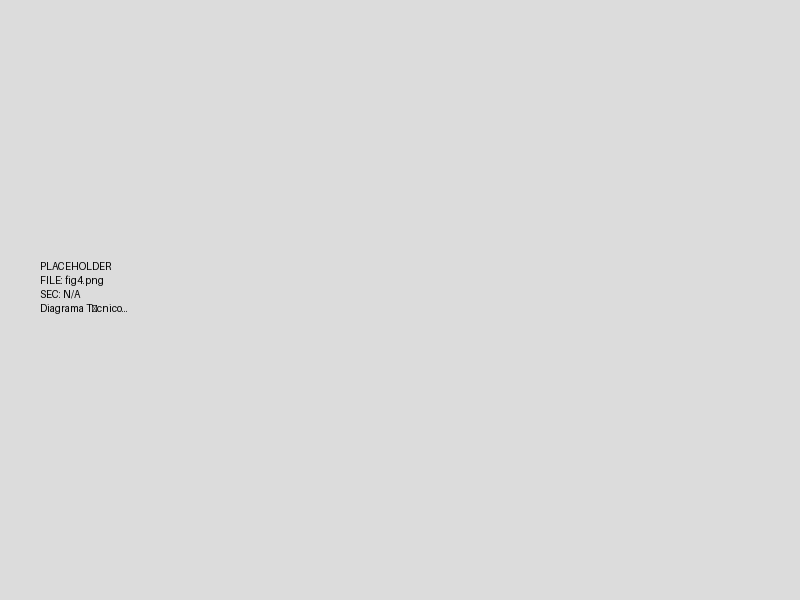
\includegraphics[width=\linewidth]{fig4.png}
\caption{Ejemplos de detección de anomalías en series temporales multivariadas del benchmark OPS-SAT. Se muestran (de arriba abajo) la señal original, puntuación de anomalía generada por el modelo y ground truth.}
\label{fig:detection_examples}
\end{figure}

En resumen, los experimentos confirman que el enfoque autosupervisado propuesto no solo alcanza métricas competitivas en precisión, sino que lo hace manteniendo características operativas esenciales para sistemas críticos espaciales. La siguiente sección discute las implicaciones más amplias de estos hallazgos.